\documentclass[ngerman]{beamer}
\usepackage[utf8]{luainputenc}
\usepackage[TS1,T1]{fontenc}
\usepackage{babel}
\usepackage{tikz}
\usetheme[pagenum,ddc]{tud}
\usepackage{xcolor}
\usepackage{listings}

\title[Präsentationsvorlagen im CD]{Präsentationsvorlagen\protect\\\mdseries im CD der TU Dresden\strut}
\subtitle{Beamer-Stil}
\author{Tobias Schlemmer}
\einrichtung{Einrichtung}
\fachrichtung{Fachrichtung}
\institut{Institut für Algebra}
\professur{Professur}
\einrichtung{}
\fachrichtung{}
\institut{}
\professur{}
\datecity{Dresden}

\newcommand*\inmm[1]{\pgfmathsetmacro\inmmwert{#1 / 1mm}\inmmwert}
\makeatletter
\newcommand*\inpt[1]{\setlength\@tempdima{#1}\the\@tempdima}
\makeatother

\AtBeginSection[]{\partpage{\usebeamertemplate***{part page}}}
\begin{document}
\section*{Vorwort}
\subsection*{Hinweis auf die Dokumentation}
% \partpage{\usebeamertemplate***{part page}}
\begin{frame}{Dokumentation}
  Die Dokumentation befindet sich in der Datei
  \url{beamer-org-mode-demo.pdf}.

  \vfill
  Es gibt Seitenzahlen und Foliennummern, die sich in diesen
  Beispiel in unterschiedlichen Stilen abwechseln. Diese Seite zeigt die Vorgabe: Folie ohne Anhang.

  \vfill
  {}\hfill los gehts\dots
\end{frame}
\setbeamertemplate{tud background}[image]{Seminarraum.jpg}%
\maketitle
\section{\textbackslash setbeamertemplate\{tud background\}[image]}

\setbeamertemplate{tud background}[image/shaded]{Seminarraum.jpg}{0.5}%
\section{\textbackslash setbeamertemplate\{tud background\}[image/shaded]}

\setbeamertemplate{tud background}[image/tikzoverlay]{Seminarraum.jpg}{%
  \node[anchor=south east] at (\tudbeamerbackgroundwidth,0) {\footnotesize Background-Art: Selbstgemalt};
}
\section{\textbackslash setbeamertemplate\{tud background\}[image/tikzoverlay]}

\setbeamertemplate{tud background}[image/shaded/tikzoverlay]{Seminarraum.jpg}{0.3}{%
  \node[anchor=south east] at (\tudbeamerbackgroundwidth,0) {\footnotesize Background-Art: Selbstgemalt};
}
\section{\textbackslash setbeamertemplate\{tud background\}[image/shaded/tikzoverlay]}

\setbeamertemplate{tud background}[image/overlay]{Seminarraum.jpg}{%
  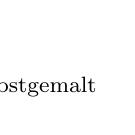
\begin{tikzpicture}%
    \useasboundingbox (0,0) -- (\tudbeamerbackgroundwidth,\tudbeamerbackgroundheight);
    \node[anchor=south east] at (\tudbeamerbackgroundwidth,0) {\footnotesize Background-Art: Selbstgemalt};
  \end{tikzpicture}%
}
\section{\textbackslash setbeamertemplate\{tud background\}[image/overlay]}

\setbeamertemplate{tud background}[image/shaded/overlay]{Seminarraum.jpg}{0.7}{%
  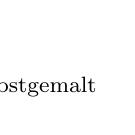
\begin{tikzpicture}%
    \useasboundingbox (0,0) -- (\tudbeamerbackgroundwidth,\tudbeamerbackgroundheight);
    \node[anchor=south east] at (\tudbeamerbackgroundwidth,0) {\footnotesize Background-Art: Selbstgemalt};
  \end{tikzpicture}%
}
\section{\textbackslash setbeamertemplate\{tud background\}[image/shaded/overlay]}

\makeatletter
\let\tstempboxa\@tempboxa
\makeatother
\setbeamertemplate{tud background}[image/pgfoverlay]{Seminarraum.jpg}{%
  \setbox\tstempboxa\hbox{%
    \begin{pgfinterruptpicture}%
      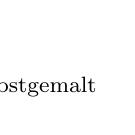
\begin{tikzpicture}%
        \useasboundingbox (0,0) -- (\tudbeamerbackgroundwidth,\tudbeamerbackgroundheight);
        \node[anchor=south east] at (\tudbeamerbackgroundwidth,0) {\footnotesize Background-Art: Selbstgemalt};
      \end{tikzpicture}%
    \end{pgfinterruptpicture}%
  }%
  \pgfqboxsynced\tstempboxa
}
\section{\textbackslash setbeamertemplate\{tud background\}[image/pgfoverlay]}

\makeatletter
\let\tstempboxa\@tempboxa
\makeatother
\setbeamertemplate{tud background}[image/shaded/pgfoverlay]{Seminarraum.jpg}{0.5}{%
  \setbox\tstempboxa\hbox{%
    \begin{pgfinterruptpicture}%
      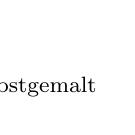
\begin{tikzpicture}%
        \useasboundingbox (0,0) -- (\tudbeamerbackgroundwidth,\tudbeamerbackgroundheight);
        \node[anchor=south east] at (\tudbeamerbackgroundwidth,0) {\footnotesize Background-Art: Selbstgemalt};
      \end{tikzpicture}%
    \end{pgfinterruptpicture}%
  }%
  \pgfqboxsynced\tstempboxa
}
\section{\textbackslash setbeamertemplate\{tud background\}[image/shaded/pgfoverlay]}

\makeatletter
\let\tstempboxa\@tempboxa
\makeatother
\setbeamertemplate{tud background}[image/pgfoverlay]{Seminarraum.jpg}{%
  \pgfsetfillopacity{0.5}%
  \usebeamertemplate{tud background shade}%
  \setbox\tstempboxa\hbox{%
    \begin{pgfinterruptpicture}%
      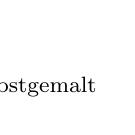
\begin{tikzpicture}%
        \useasboundingbox (0,0) -- (\tudbeamerbackgroundwidth,\tudbeamerbackgroundheight);
        \node[anchor=south east] at (\tudbeamerbackgroundwidth,0) {\footnotesize Background-Art: Selbstgemalt};
      \end{tikzpicture}%
    \end{pgfinterruptpicture}%
  }%
  \pgfqboxsynced\tstempboxa
}
\section{\textbackslash setbeamertemplate\{tud background\}[image/pgfoverlay]+
\textbackslash usebeamertemplate{tud background shade}}

\end{document}
%%% Local Variables: 
%%% mode: latex
%%% TeX-master: t
%%% End: 
